\section{Hyperparameters}
\label{parameters}
This section proposes an equation to evaluate the build-trace trade-off of the PHR algorithm. Two possible solutions for the optimization problem are them presented in the form of grid search and Bayesian optimization. As established in the previous section, PHR depends on the parameters $\alpha$ and $\delta$ describing initial cut size and shrink rate. These parameters can be set to adjust the trade-off between build time and trace performance. However, the optimal parameters can differ between scenes and view points, especially when dealing with dynamic scenes and refitted auxiliary trees.
% TODO: Add figure that shows different optimal parameters and prove thesis
Frame size also plays a role as higher resolutions profit more from well optimized bounding volume hierarchies while the hit taken by the extended build time is not as significant given the overall higher computational effort. 
\subsection{Evaluation}
\label{evaluation}
Ultimately, the overall frame time including BVH build time and render duration needs to be minimized to unlock the full potential of progressive hierarchical refinement. Stopping the actual execution times is neither efficient nor reliable enough, so an efficient metric that makes the trade-off quantifiable is needed. 

A number of metrics have been proposed to estimate the quality of a given bounding volume hierarchy. A well known cost model based on the surface area heuristic, taken from \cite{meister21survey}, is given by the recurrence equation 
\[
c(N) =  
    \begin{cases}
        c_T + \sum_{N_c}P(N_c|N)c(N_c) &\quad\text{if }N\text{ is interior node,}\\
        c_I|N|&\quad\text{otherwise}\\
    \end{cases}
\]
where $C(N)$ is the cost of the subtree with root $N$, $N_c$ is a child of node $N$, $P(N_c|N)$ is the conditional probability of traversing node $N_c$ when $N$ is hit and $|N|$ is the number of primitives in the subtree with root $N$. 

Constants $c_T$ and $c_I$ express the average cost of a traversal step and ray-primitive intersection, respectively. Utilizing the micro-benchmarking capabilities of Go revealed that a triangle intersection takes approximately 7 nanoseconds on average, while a traversal step takes around 12 nanoseconds. Consequently, these constants are set to $c_T = 2$ and $c_I = 1$, roughly representing the ratios between those values. 
The conditional probabilities of traversing a node are expressed using the surface area heuristic\cite{goldsmith_automatic_1987,macdonald_heuristics_1990}
\[
P(N_c|N)^{SAH} = \frac{SA(N_c)}{SA(N)}
\]
where $SA(N)$ and $SA(N_c)$  are the bounding box surface areas of nodes $N$ and $N_c$, respectively. 

Evaluating the build complexity of PHR given a set of parameters and an arbitrary scene is not as trivial, as there is no clear correlation between the parameter values and associated build times.  
\begin{figure}
    \centering
    \subcaptionbox{Build Time}{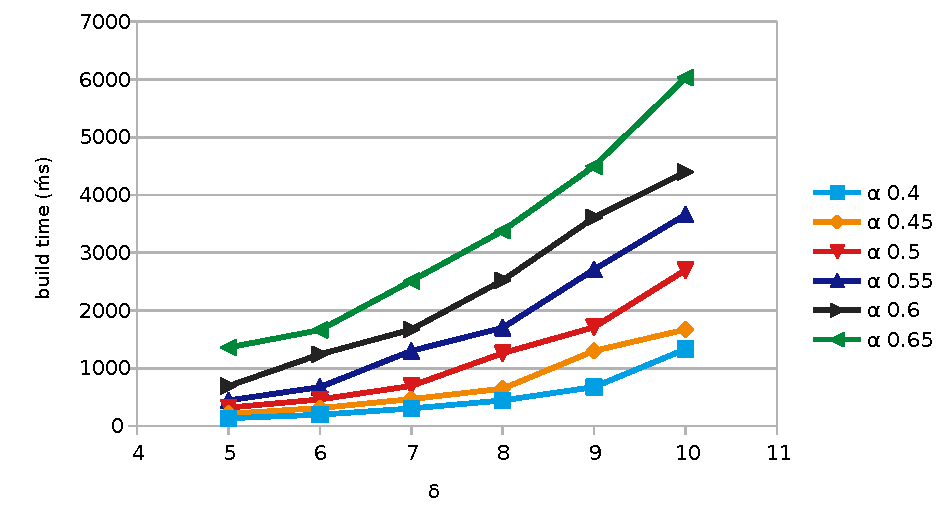
\includegraphics[width=0.45\textwidth]{images/build_time.pdf}}
    \hfill
    \subcaptionbox{Build Cost}{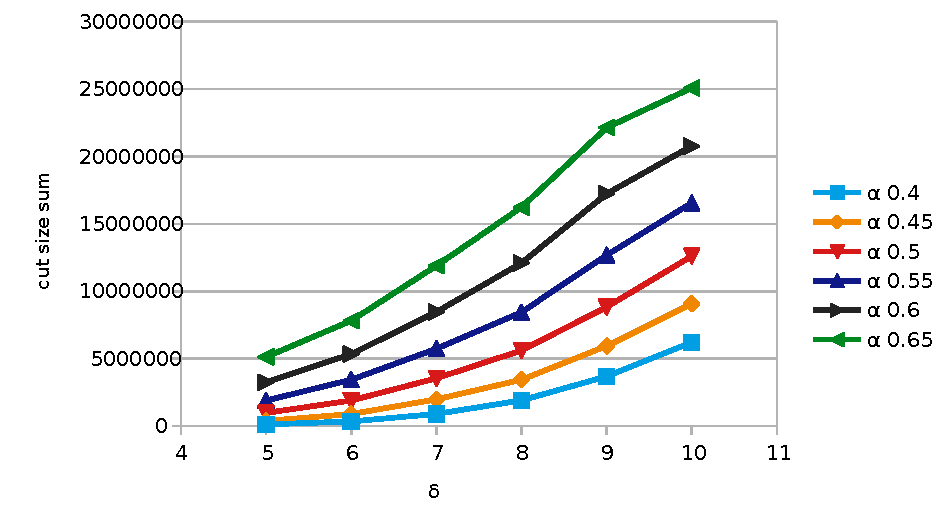
\includegraphics[width=0.45\textwidth]{images/build_cost.pdf}}
    \caption{Both the build time and corresponding build cost for the San Miguel scene. This corresponds to a correlation of 0.994.}
    \label{fig:build_cost}
\end{figure}
For scenes with medium to high complexity, the tree size of the resulting BVH could be used as a metric with an average correlation coefficient of around 0.98 between tree size and build time. This correlation does not hold true for simpler scenes though, as trees stop growing once no favorable splits can be found anymore.
A better metric is the total sum of all cut sizes, as seen in figure \ref{fig:build_cost}, which can be obtained through a minimal adjustment of the progressive hierarchical refinement algorithm. The surface area heuristic evaluation is the most expensive part of PHR and thus the total number of evaluated nodes directly correlates with the execution duration. Using an atomic counter, the performance penalty is very marginally to non existing. Furthermore, an alternative implementation can be used for the optimization process. The correlation between this number and the BVH construction time averages to 0.99 across all tested scenes.

Let the build cost $b$ be defined as
\[
    b(\alpha, \delta) = \sum_{cut\in PHR'(\alpha, \delta)}|cut|
\]
where $b(\alpha, \delta)$ is cost of a PHR execution given the parameters $\alpha$ and $\delta$, $PHR'(\alpha, \delta)$ is a execution of the progressive hierarchical refinement algorithm resulting in a set of all cuts processed and $|cut|$ is the length of given cut.

I propose an equation to evaluate the combined cost of a frame rendered using the PHR algorithm, which also factors in the build-trace trade-off. Given a pair of parameters $\alpha$ and $\delta$, this cost is defines as
\[
    e(\alpha,\delta) = ||b(\alpha,\omega)|| + \omega^2 ||c(PHR(\alpha,\omega))||
\]
with $||b(\alpha,\delta)||$ being the normalized build cost and $||c(PHR(\alpha,\omega))||$ the normalized SAH cost of the resulting BVH. The coefficient $\omega$ functions as a weight determining to what extend trace performance should be favored over build duration. For $\omega=1$, both trace and build performance are weighed equally, $\omega>1$ favors higher trace speed and $\omega<1$ encourages faster build times. These trade-off depends on scene complexity and frame size, so $\omega$ is defined as:
\[
    \omega = (\frac{|prim|}{\omega_p})^2 * (\frac{w*h}{\omega_r})
\]
where $|prim|$ is the total number of primitives in the scene and $w$ and $h$ are width and height of the rendered frame, respectively. $\omega_p$ and $\omega_r$ are constants depending on the performance of the used path tracer and the targeted frame rate, so they stay constant across all scenes. $\omega_p$ expresses a number of primitives and $\omega_r$ a frame size at which the trade-off should be equal, i.e. $\omega=1$. Once those numbers are exceeded, BVH quality is favored increasingly. 

Combining the equation with the previously mentioned metrics and given a search space over the parameters $\alpha$ and $\delta$ (e.g. $\alpha\in A=[0.4,0.6], \delta\in D=[5,10]$) leads to the expression:
\[
    e(\alpha,\delta) =
        \frac{b(\alpha, \delta)}
        {\max_{\alpha\in A,\delta\in D}b(\alpha, \delta)}
        + \omega^2
        \frac{c(PHR(\alpha, \delta))}
        {\max_{\alpha\in A,\delta\in D}c(PHR(\alpha, \delta))}
\]
where $PHR(\alpha,\delta)$ is a execution of the PHR algorithm using the parameters $\alpha$ and $\delta$ resulting in the root node of a bounding volume hierarchy.
\clearpage
\subsection{Grid Search}
The brute force approach grid search is the obvious first choice to solve this optimization problem. A number of possible values is chosen for each parameter (e.g. $\alpha\in\{0.45,0.5,0.55\}$ $\delta\in\{5,6,7,8\}$) and all possible combinations are tested and evaluated. By postponing the evaluation of $e(\alpha,\delta)$ until all individual cost evaluations $b(\alpha, \delta)$ and $c(PRH(\alpha,\delta))$ are available makes their maxima directly accessible, which is another advantage of grid search. 

Usually, grid search would be too costly for such a time critical task. In this case however, only two parameters need to be optimized and the search space is relatively small making grid search a potentially viable approach. 

\subsection{Bayesian Optimization}
A more efficient approach compared to grid search is Bayesian optimization\cite{pelikan99boa}, which explores the search space by taking previous observations into account. This is done by placing a prior probability distribution over the objective function $e(\alpha,\delta)$. First, parameters $\alpha$ and $\delta$ are chosen by random in the given search space. Following their evaluation, the prior is updated to form a posterior distribution. Based on this posterior distribution, an acquisition function is constructed to select the next point worth exploring. 

In particular, the Bayesian optimizer\cite{ou19bo} utilizes a Gaussian process to define the prior/posterior distribution, and expected improvement is used as exploration strategy.

One issue compared to the aforementioned grid search approach is, that the maximum BVH and build costs are not directly available when evaluating $e(\alpha,\delta)$. This is solved by running PHR once with the lowest possible parameters in the search space to obtain the maximum BVH cost and once with the highest possible parameters to obtain the maximum build cost. These numbers correspond to the respective maxima very reliably and there evaluations can also be factored into the prior probability distribution.
\cleardoublepage